%\section{Experimente}

%Unterscheidung zwischen männlein und weiblein

%Laufzeit Training, Prädiktion


\newpage
\section{GUI}

Zur besseren Bedienbarkeit des Programms wurde eine graphische Benutzeroberfläche entwickelt.
Diese ermöglicht es mit geringem Aufwand, Modelle aus den vorhandenen Merkmalsvektorfolgen zu trainieren sowie zu testen.
%Konfigurationen zu tätigen und die gewünschten Funktionen zu starten.
Hierdurch wird der Umgang mit den Datenmengen sowie die Durchführung von Experimenten vereinfacht. % das Erzeugen von Grafiken und Auswertungen. 
Die Benutzeroberfläche ist in der Abbildung \ref{fig:gui} dargestellt.


\medskip
\begin{figure}[tbph!]
\centering
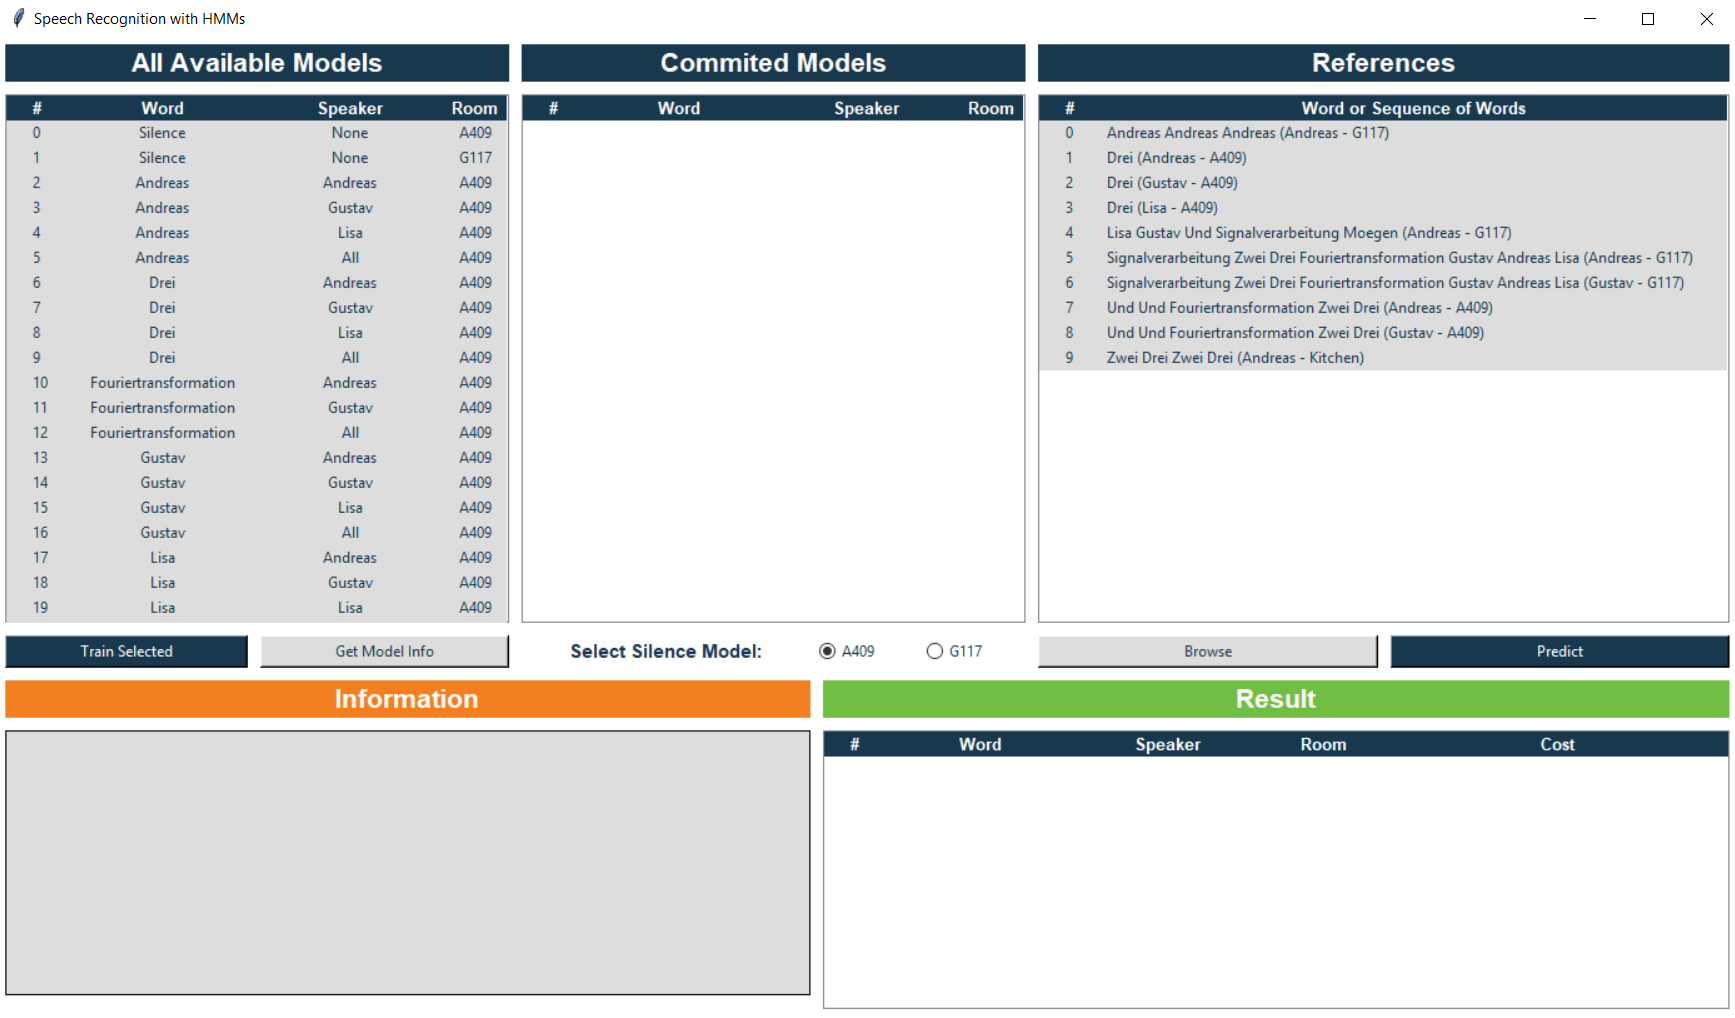
\includegraphics[width=0.92\linewidth]{grafic/gui}
\caption{grafische Benutzeroberfläche}
\label{fig:gui}
\end{figure}


In der linken oberen Box sind alle verfügbaren Modelle aufgelistet.
Über die beiden darunter liegenden Buttons können die Modelle entweder neu trainiert oder Informationen, wie z.B. die Modelllänge oder die benötigten Iterationen, angezeigt werden.
Die mittlere Box zeigt die aktuell für die Klassifikation zur Auswahl stehenden Modelle an.
Durch einen Doppelklick auf ein Modell in der linken Box, kann dieses für die später folgende Prädiktion geladen werden.
Das zu verwendende Stillemodell wird über die darunter angeordneten Radiobuttons ausgewählt.

Um ein Wort durch die Software klassifizieren zu lassen, muss dieses durch den Button \en{Browse} in die obere rechte Box geladen und ausgewählt werden.
Hierdurch können auch gesprochene Wortfolgen ausgewertet werden.
Zum Starten der Prädiktion wird der Button \en{Predict} betätigt, das Ergebnis wird danach rechts unten angezeigt.
Hierbei wird sowohl das erkannte Wort, als auch der ermittelte Sprecher und die benötigten Kosten aufgelistet. 





% wortfolgen laden und testen
% informationen zu modellen 
% stille modell 
% kosten anschauen



